\documentclass[14pt,a4paper]{extreport}

\usepackage[left=30mm, top=20mm, right=10mm, bottom=20mm]{geometry}
\usepackage{cmap}		
\usepackage[utf8]{inputenc}
\usepackage[english, russian]{babel}
\usepackage{framed}
\usepackage{amsmath}
\usepackage{graphicx}
\usepackage{wrapfig}
\usepackage{verbatim}
\usepackage{indentfirst}
\usepackage{textcomp}
\usepackage{titlesec}
\usepackage{alltt}
\usepackage{float}
\usepackage{cite}
\usepackage{url}
\usepackage{listings}
\usepackage{color}

\lstset{
    language=C++,
    basicstyle=\ttfamily,
    keywordstyle=\color{blue}\ttfamily,
    stringstyle=\color{red}\ttfamily,
    commentstyle=\color{green}\ttfamily,
    morecomment=[l][\color{magenta}]{\#}
}
%%%%%%%%%%%%%%%%%%%%%%%%%%%%%%%%%%%%%%%%%%%%%%%%%%%%%%%%%%%%%%%%%%%%%%%%

\titleformat{\chapter}[display]
    {\filcenter\large\bfseries}
    {\MakeUppercase{\chaptertitlename} \thechapter}
    {8pt}
    {\bfseries}{}
\titleformat{\section}
    {\normalsize\bfseries}
    {\thesection}
    {1em}{}
\titleformat{\subsection}
    {\normalsize\bfseries}
    {\thesubsection}
    {1em}{}

%% Настройка вертикальных и горизонтальных отступов
\titlespacing*{\chapter}{0pt}{-30pt}{8pt}
\titlespacing*{\section}{\parindent}{*4}{*4}
\titlespacing*{\subsection}{\parindent}{*4}{*4}

%% Отступ от левого края
\oddsidemargin=0pt 

\newcommand{\HRule}{\rule{\linewidth}{0.5mm}}

\begin{document}

%% Титульный
%%%%%%%%%%%%%%%%%%%%%%%%%%%%%%%%%%%%%%%%%%%%%%%%%%%%%%%%%%%%%%%%%%%%%%%%
\begin{titlepage}
\begin{center}


{\normalsize 
Федеральное государственное автономное образовательное учреждение высшего образования 
\\Санкт-Петербургский национальный исследовательский университет 
\\информационных технологий, механики и оптики}

\vspace{1.5cm}

\vspace{0.5cm}
\large Факультет систем управления и робототехники
% Upper part of the page. The '~' is needed because \\
% only works if a paragraph has started.
%\includegraphics[width=0.18\textwidth]{img/logo.png}~\\[1cm]
\vspace{2cm}

\large Курсовой проект
\\ Вариант №2

по дисциплине <<Программирование систем управления>>

{ \large \bfseries <<Моделирование системы управления>>\\[0.4cm] }

% Author and supervisor
\noindent

\begin{flushright} \normalsize
\emph{Выполнили:}\\
Студент группы R41332\\
Волков \textsc{А.~А.}\\
% Щербаков \textsc{П.~В.}\\

\emph{Проверил:} \\
Томашевич \textsc{С.~И.}
\end{flushright}

\vfill

% Bottom of the page
{\normalsize Санк-Петербург, 2019 г.}

\end{center}
\end{titlepage}

%%%%%%%%%%%%%%%%%%%%%%%%%%%%%%%%%%%%%%%%%%%%%%%%%%%%%%%%%%%%%%%%%%%%%%%%

%% Оглавление
%%%%%%%%%%%%%%%%%%%%%%%%%%%%%%%%%%%%%%%%%%%%%%%%%%%%%%%%%%%%%%%%%%%%%%%%
\newpage
\tableofcontents
%%%%%%%%%%%%%%%%%%%%%%%%%%%%%%%%%%%%%%%%%%%%%%%%%%%%%%%%%%%%%%%%%%%%%%%%

%% Задание
%%%%%%%%%%%%%%%%%%%%%%%%%%%%%%%%%%%%%%%%%%%%%%%%%%%%%%%%%%%%%%%%%%%%%%%%
\chapter*{Задание}
\addcontentsline{toc}{chapter}{Задание}

\begin{enumerate}
\item
Реализовать класс интегратора в .cpp и .h файлах.
    
\item 
Привести задающее воздействие в виде модели с использованием интегратором.
    
\item 
Дисретизировать полученные модели задающего воздействия 
и объекта управления с шагами дискретизации 5, 50, 100 Гц.

\item
Программно реализовать отдельными классами четыре случая объектов 
(непрерывный и три дискретных). Для дискретных случаев сделать 
реализацию с использованием разностных уравнений.
\begin{equation} 
    x_{k+1} = A \cdot x_k
\end{equation}
То есть интегратор заменяется на элемент памяти.

\item 
Добавить реализованные классы в предоставленную программу для \\ QtCreator.

\item
Поочередно провести сравнение поведений реализованных непрерывв-
ных моделей с дискретными моделями с соответствующими шагами
дискретизации. Шаг дискретизации меняется в предоставленной про-
грамме. В результате должно получиться три пары сравнений.

\item 
В предоставленной программе QtCreator настроить последовательный
порт (qSerialPort) на скорость 115200 бод, формат 8N1.

\item 
Закодировать с помощью метода COBS значения, полученные с выхода
объекта в следующем формате:
{[0x0A 0xXX 0xXX 0xXX 0xXX 0xCR]}, где 0xXX – байты полученного 
числа с плавающей точкой (float) в
обратном порядке, а 0xCR – проверочная сумма, равная сумме всех
остальных байт сообщения, вычтенной из 0xFF.

\end{enumerate}
%%%%%%%%%%%%%%%%%%%%%%%%%%%%%%%%%%%%%%%%%%%%%%%%%%%%%%%%%%%%%%%%%%%%%%%%

%% Исходные данные
%%%%%%%%%%%%%%%%%%%%%%%%%%%%%%%%%%%%%%%%%%%%%%%%%%%%%%%%%%%%%%%%%%%%%%%%
\newpage
\chapter*{Исходные данные}
\addcontentsline{toc}{chapter}{Исходные данные}

Входной сигнал задается в следующем виде:
\begin{equation}
    u(t) = 3 \cdot  \cos{(0.1 \cdot t + 1)}
\end{equation}

Система представлена в виде Вход-Состояние-Выход. Матрицы A, B, C выглядят следующим образом:
\begin{equation}
    A = 
    \begin{bmatrix} 
        0 & 1 & 0 \\ 
        0 & 0 & 1 \\
        -1.5 & -5 & -2
    \end{bmatrix}
\end{equation}

\begin{equation}
    B = 
    \begin{bmatrix} 
        0 \\
        0 \\
        1
    \end{bmatrix}
\end{equation}

\begin{equation}
    C = 
    \begin{bmatrix} 
        0.5 & 0 & 0
    \end{bmatrix}
\end{equation}

Расчет выходного сигнала проходит по следующим формулам:
\begin{equation}
\dot x(t) = A \cdot x(t) + B \cdot u(t)
\end{equation}

\begin{equation}
y(t) = C \cdot x(t)
\end{equation}
%%%%%%%%%%%%%%%%%%%%%%%%%%%%%%%%%%%%%%%%%%%%%%%%%%%%%%%%%%%%%%%%%%%%%%%%

%% Ход работы
%%%%%%%%%%%%%%%%%%%%%%%%%%%%%%%%%%%%%%%%%%%%%%%%%%%%%%%%%%%%%%%%%%%%%%%%
\chapter*{Ход работы}
\addcontentsline{toc}{chapter}{Ход работы}
Исходный код программы представлен в приложении А. 

Непрерывная система отличается от дискретной отличается способом 
расчета вектора состояния и параметрами системы. Переходные процессы для дискретной и непрерывной системы отличаются 
только в случае очень большого шага дискретизации.

Поскольку задающее воздействие считается с шагом дискретизации,
то для его расчета использовалась реализация с помощью двух интеграторов
с заданной обратной связью.

Интегратор реализован с помощью метода левых прямоугольников:
\begin{equation}
    y_{k+1} = y_{k} + x \cdot \Delta t
\end{equation}

Для получения сигнала косинуса два интегратора 
соединяются последовательно и замыкаются отрицательной обратной связью
с коэфициентом равным квадрату частоты. Начальная фаза устанавливается
при помощи начальных условий интеграторов. В логике программного кода - 
величиной предыдущего состояния.

Ниже приведены параметры системы в случае шага дискретизации 5 Гц.

\begin{equation}
    A_{d} = 
    \begin{bmatrix} 
        0.998 & 0.193 & 0.017 \\ 
        -0.026 & 0.911 & 0.159 \\
        -0.238 & -0.819 & 0.594
    \end{bmatrix}
\end{equation}

\begin{equation}
    B_{d} = 
    \begin{bmatrix} 
        0.001 \\ 
        0.0173 \\
        0.159
    \end{bmatrix}
\end{equation}

\begin{equation}
    C_{d} = 
    \begin{bmatrix} 
        0.5 & 0 & 0
    \end{bmatrix}
\end{equation}

Далее приведены параметры системы в случае шага дискретизации 50 Гц.

\begin{equation}
    A_{d} = 
    \begin{bmatrix} 
        1.000 & 0.020 & 0.000 \\ 
        0.000 & 0.999 & 0.020 \\
        -0.029 & -0.098 & 0.960
    \end{bmatrix}
\end{equation}

\begin{equation}
    B_{d} = 
    \begin{bmatrix} 
        0.000 \\ 
        0.000 \\
        0.0196
    \end{bmatrix}
\end{equation}

\begin{equation}
    C_{d} = 
    \begin{bmatrix} 
        0.5 & 0 & 0
    \end{bmatrix}
\end{equation}

Далее приведены параметры системы в случае шага дискретизации 100 Гц.

\begin{equation}
    A_{d} = 
    \begin{bmatrix} 
        1.000 & 0.010 & 0.000 \\ 
        0.000 & 1.000 & 0.010 \\
        -0.015 & -0.050 & 0.980
    \end{bmatrix}
\end{equation}

\begin{equation}
    B_{d} = 
    \begin{bmatrix} 
        0.000 \\ 
        0.000 \\
        0.001
    \end{bmatrix}
\end{equation}

\begin{equation}
    C_{d} = 
    \begin{bmatrix} 
        0.5 & 0 & 0
    \end{bmatrix}
\end{equation}

Переходной процесс непрерывной системы с шагом дискретизации 
5 Гц представлен на рис.\ref{fig:con_5hz}.
\begin{figure}[H]
    \centering
    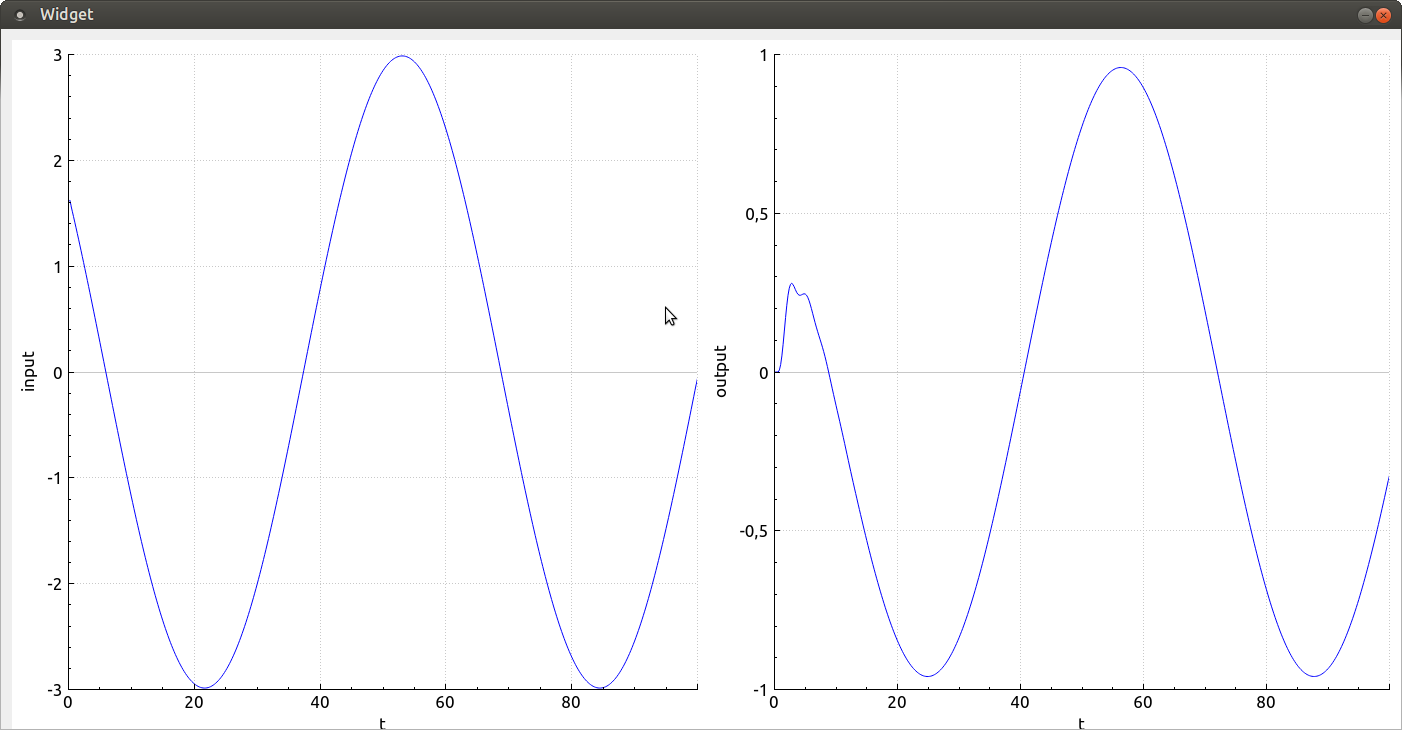
\includegraphics[width=160mm]{img/con_5hz.png}
    \caption{Переходной процесс непрерывной системы с шагом дискретизации 5 Гц}
    \label{fig:con_5hz}
\end{figure}

Переходной процесс дискретной системы с шагом дискретизации 
5 Гц представлен на рис.\ref{fig:dis_5hz}.
\begin{figure}[H]
    \centering
    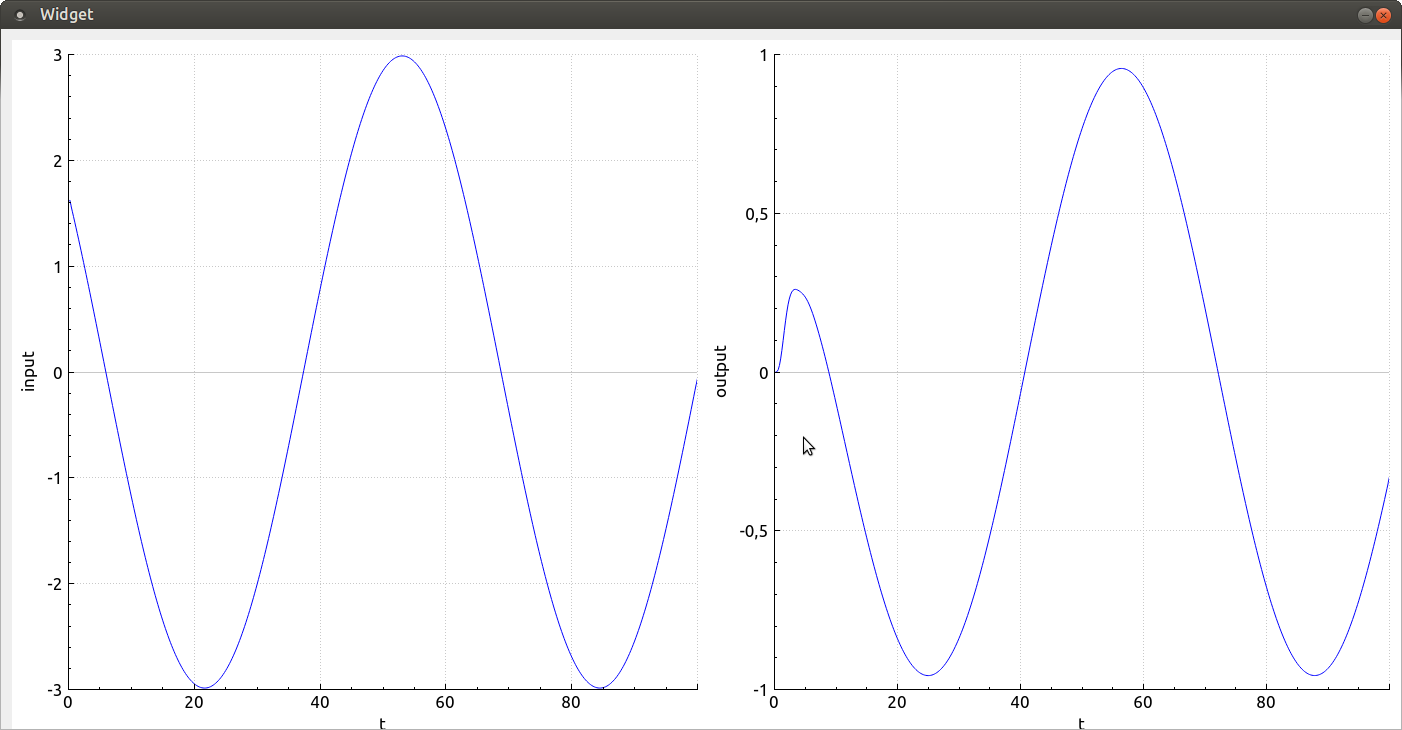
\includegraphics[width=160mm]{img/dis_5hz.png}
    \caption{Переходной процесс дискретной системы 
    с шагом дискретизации 5 Гц}
    \label{fig:dis_5hz}
\end{figure}

Переходной процесс непрерывной системы с шагом дискретизации 
50 Гц представлен на рис.\ref{fig:con_50hz}.
\begin{figure}[H]
    \centering
    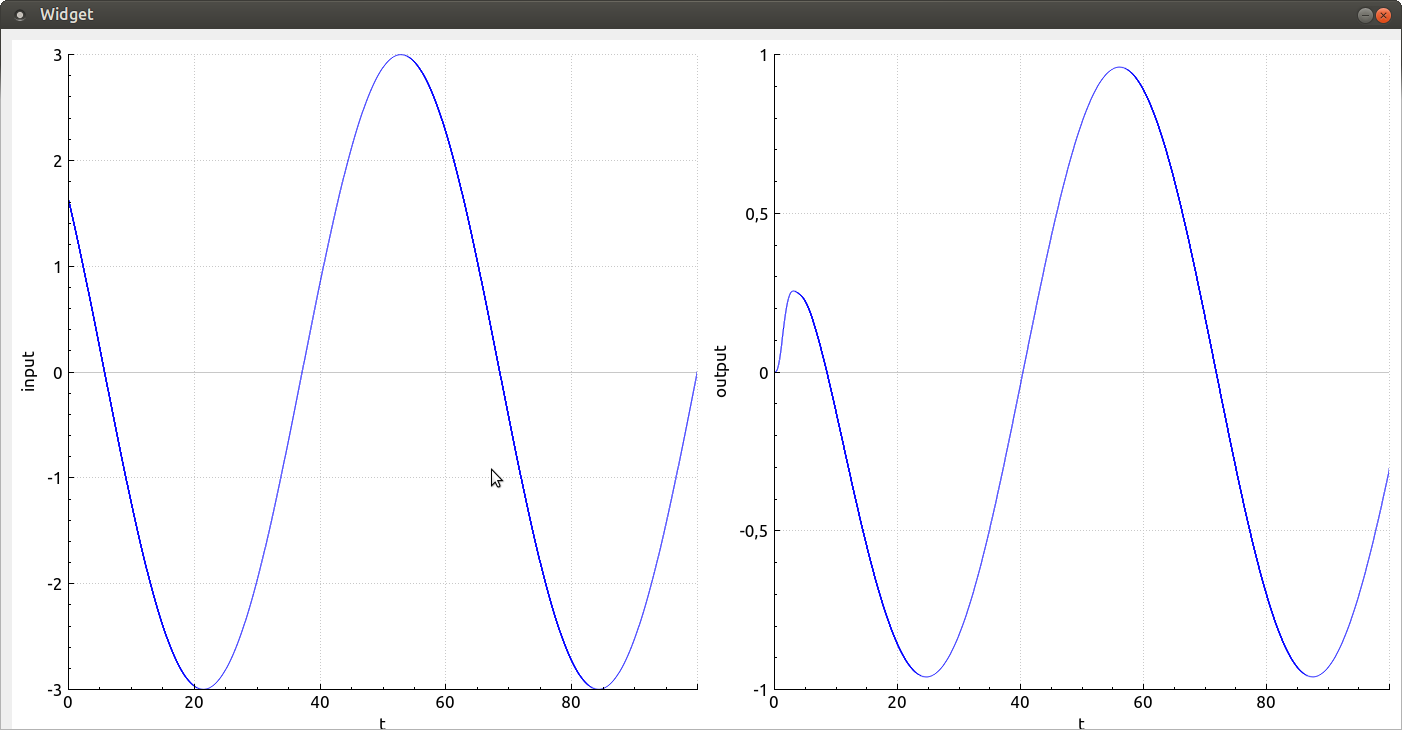
\includegraphics[width=160mm]{img/con_50hz.png}
    \caption{Переходной процесс непрерывной системы с шагом дискретизации 5 Гц}
    \label{fig:con_50hz}
\end{figure}

Переходной процесс дискретной системы с шагом дискретизации 
50 Гц представлен на рис.\ref{fig:dis_50hz}.

\begin{figure}[H]
    \centering
    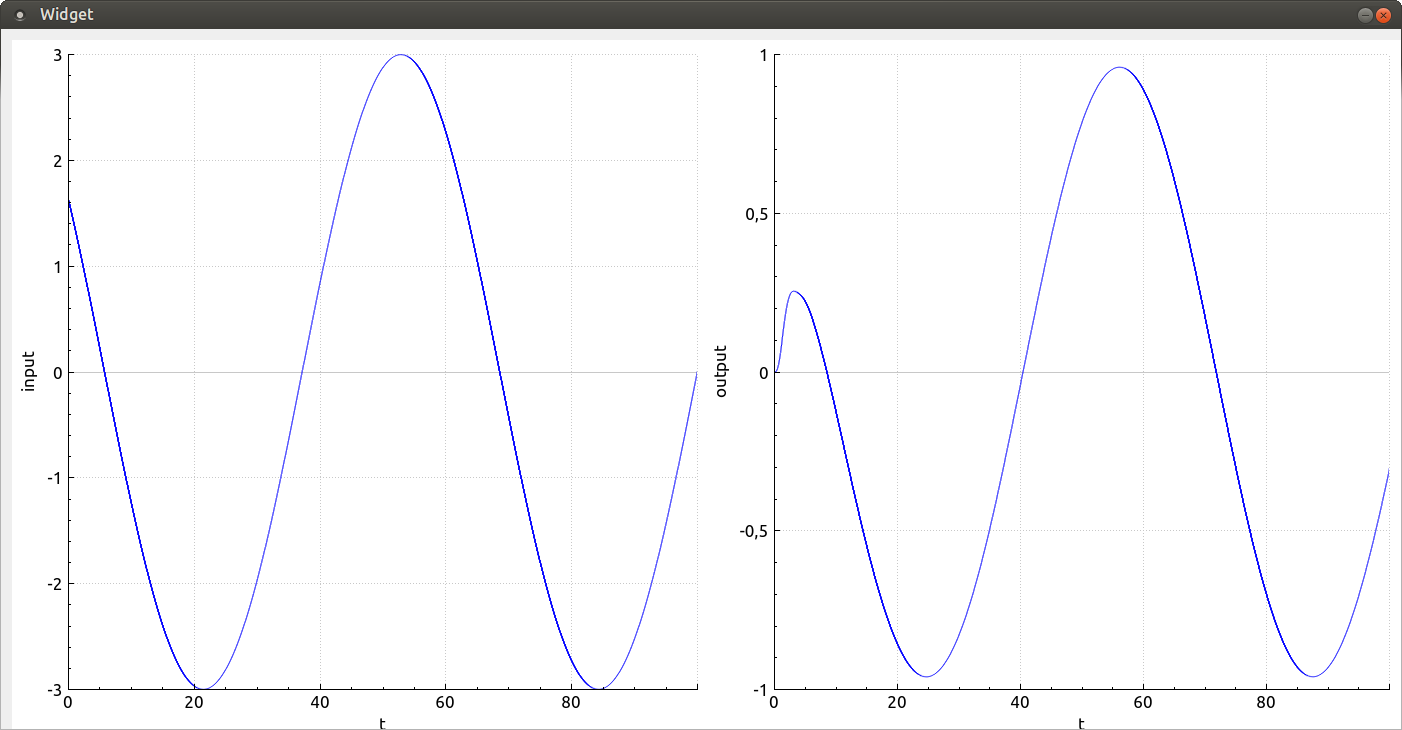
\includegraphics[width=160mm]{img/dis_50hz.png}
    \caption{Переходной процесс дискретной системы 
    с шагом дискретизации 50 Гц}
    \label{fig:dis_50hz}
\end{figure}

Переходной процесс непрерывной системы с шагом дискретизации 
100 Гц представлен на рис.\ref{fig:con_100hz}.
\begin{figure}[H]
    \centering
    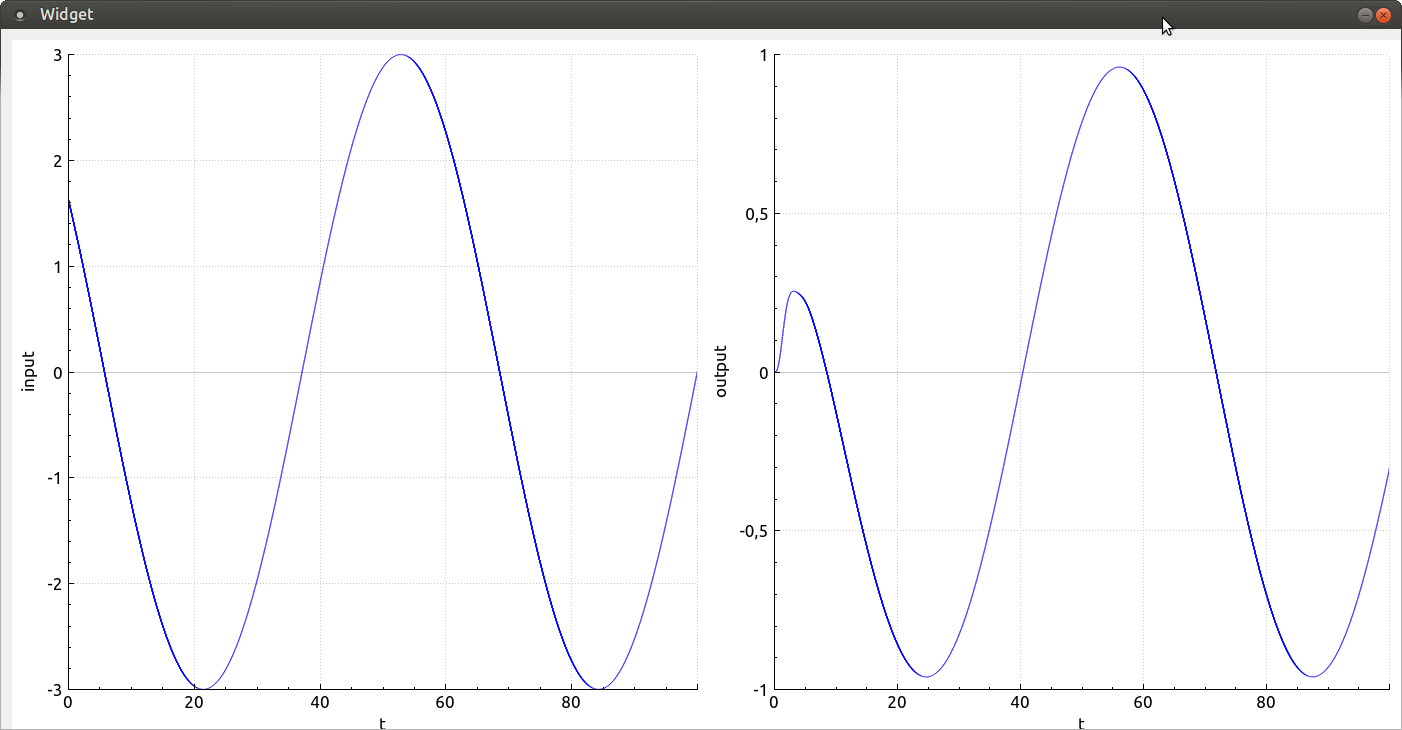
\includegraphics[width=160mm]{img/con_100hz.png}
    \caption{Переходной процесс непрерывной системы с шагом дискретизации 5 Гц}
    \label{fig:con_100hz}
\end{figure}

Переходной процесс дискретной системы с шагом дискретизации 
100 Гц представлен на рис.\ref{fig:dis_100hz}.

\begin{figure}[H]
    \centering
    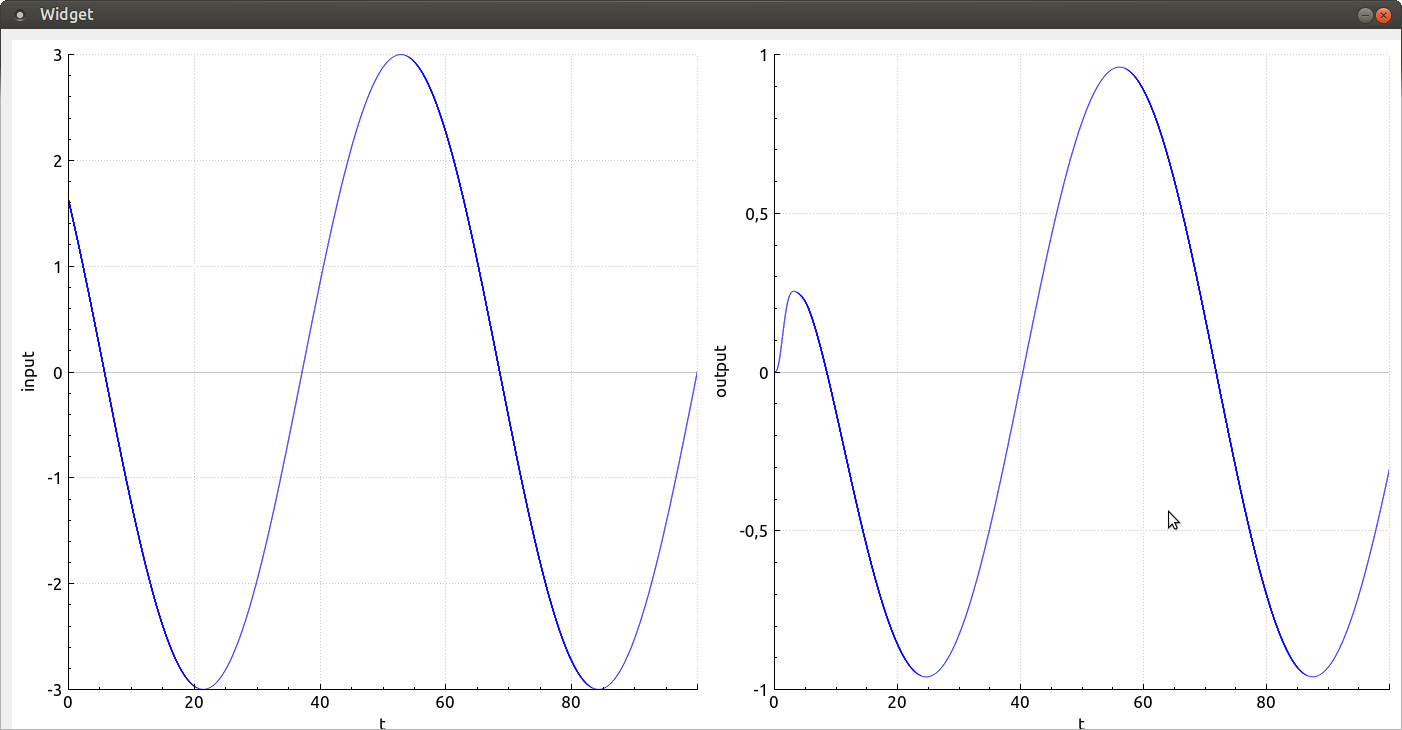
\includegraphics[width=160mm]{img/dis_100hz.png}
    \caption{Переходной процесс дискретной системы 
    с шагом дискретизации 100 Гц}
    \label{fig:dis_100hz}
\end{figure}

Для проверки работы UART был эмулирован терминал OS Linux, в который было отправлено тестовое значение 
42.0 используя заданные параметры передачи данных. 
Результат отправки представлен на рис.\ref{fig:uart}.
\begin{figure}[H]
    \centering
    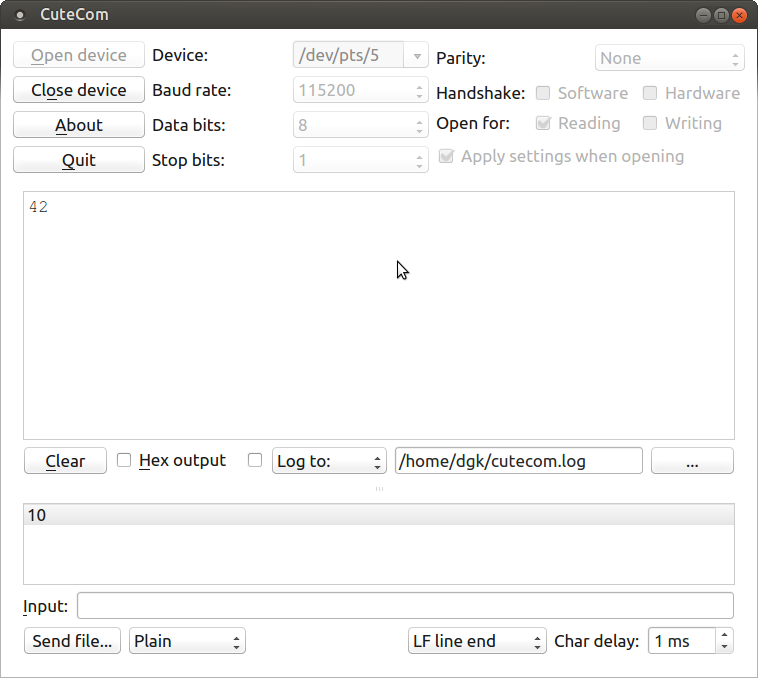
\includegraphics[width=160mm]{img/uart.png}
    \caption{Отправка сигнала по UART}
    \label{fig:uart}
\end{figure}

Кодировка сигнала происходит с помощью стороннего заголовочного файла. 
Результат кодировки сигнала 42.0 представлен на рис.\ref{fig:cobs}.
\begin{figure}[H]
    \centering
    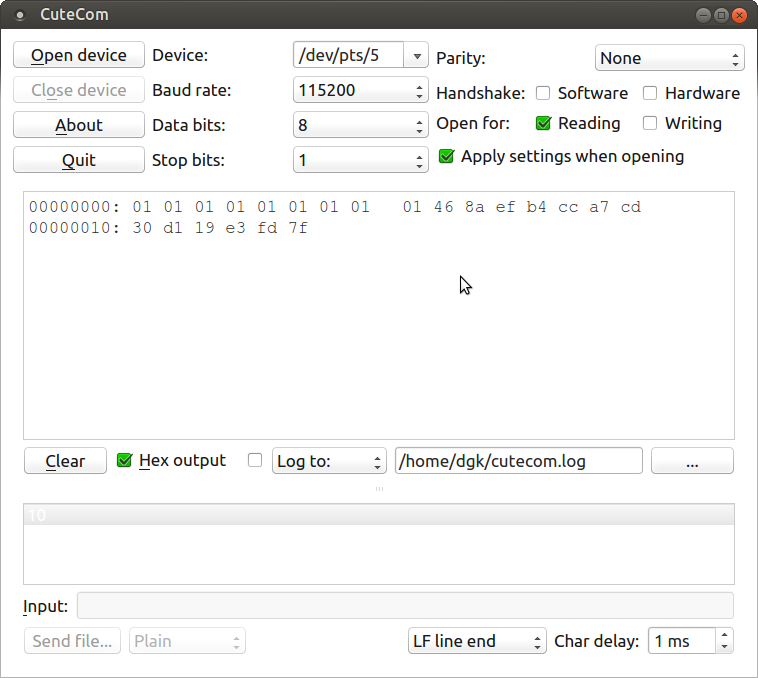
\includegraphics[width=160mm]{img/cobs.png}
    \caption{Отправка зашифрованного сигнала}
    \label{fig:cobs}
\end{figure}
%%%%%%%%%%%%%%%%%%%%%%%%%%%%%%%%%%%%%%%%%%%%%%%%%%%%%%%%%%%%%%%%%%%%%%%%

%% Вывод
%%%%%%%%%%%%%%%%%%%%%%%%%%%%%%%%%%%%%%%%%%%%%%%%%%%%%%%%%%%%%%%%%%%%%%%%
\chapter*{Вывод}
\addcontentsline{toc}{chapter}{Вывод}

В ходе работы была промоделирован объект управления в виде вход-состояние-выход 
с помощью программы, написанной на языке C++. При этом объект управления
был представлен в четырех исполнениях: непрерывный и три дискретных с 
различными шагами дискретизации. По итогу было получено, что основную
роль в адекватности моделирования играет величина шага дискретизации.
При увеличении шага точность моделирования падает, график переходного
процесса становится "ломаным". И на определенном этапе выходной процесс
становится неустойчивым.

%%%%%%%%%%%%%%%%%%%%%%%%%%%%%%%%%%%%%%%%%%%%%%%%%%%%%%%%%%%%%%%%%%%%%%%%

%% Приложение А. Исходный код программы
%%%%%%%%%%%%%%%%%%%%%%%%%%%%%%%%%%%%%%%%%%%%%%%%%%%%%%%%%%%%%%%%%%%%%%%%
\newpage
\chapter*{Приложение А. Исходный код программы}
\addcontentsline{toc}{chapter}{Приложение А. Исходный код программы}

\lstinputlisting[language=C++, caption=Файл model.h]{./../src/qt/model/model.h}
\lstinputlisting[language=C++, caption=Файл model.cpp]{./../src/qt/model/model.cpp}
\lstinputlisting[language=C++, caption=Файл integrator.h]{./../src/qt/model/integrator.h}
\lstinputlisting[language=C++, caption=Файл integrator.cpp]{./../src/qt/model/integrator.cpp}
\lstinputlisting[language=C++, caption=Файл matrix.h]{./../src/qt/model/matrix.h}
\lstinputlisting[language=C++, caption=Файл matrix.cpp]{./../src/qt/model/matrix.cpp}
\lstinputlisting[language=C++, caption=Файл main.cpp]{./../src/qt/main.cpp}
\lstinputlisting[language=C++, caption=Файл widget.h]{./../src/qt/view/widget.h}
\lstinputlisting[language=C++, caption=Файл widget.cpp]{./../src/qt/view/widget.cpp}
\lstinputlisting[language=C++, caption=Файл cobs.h]{./../src/qt/model/cobs.h}

%%%%%%%%%%%%%%%%%%%%%%%%%%%%%%%%%%%%%%%%%%%%%%%%%%%%%%%%%%%%%%%%%%%%%%%%

\end{document}
